\documentclass[12pt]{article}
\usepackage{graphicx}
\usepackage[utf8]{inputenc}


\title{List of Style}

\begin{document}
\maketitle



\section{Watercolor}

\subsection*{Description}

This technic use water soluble ink applied with a brush.

\begin{figure}[!ht]
    \begin{center}
        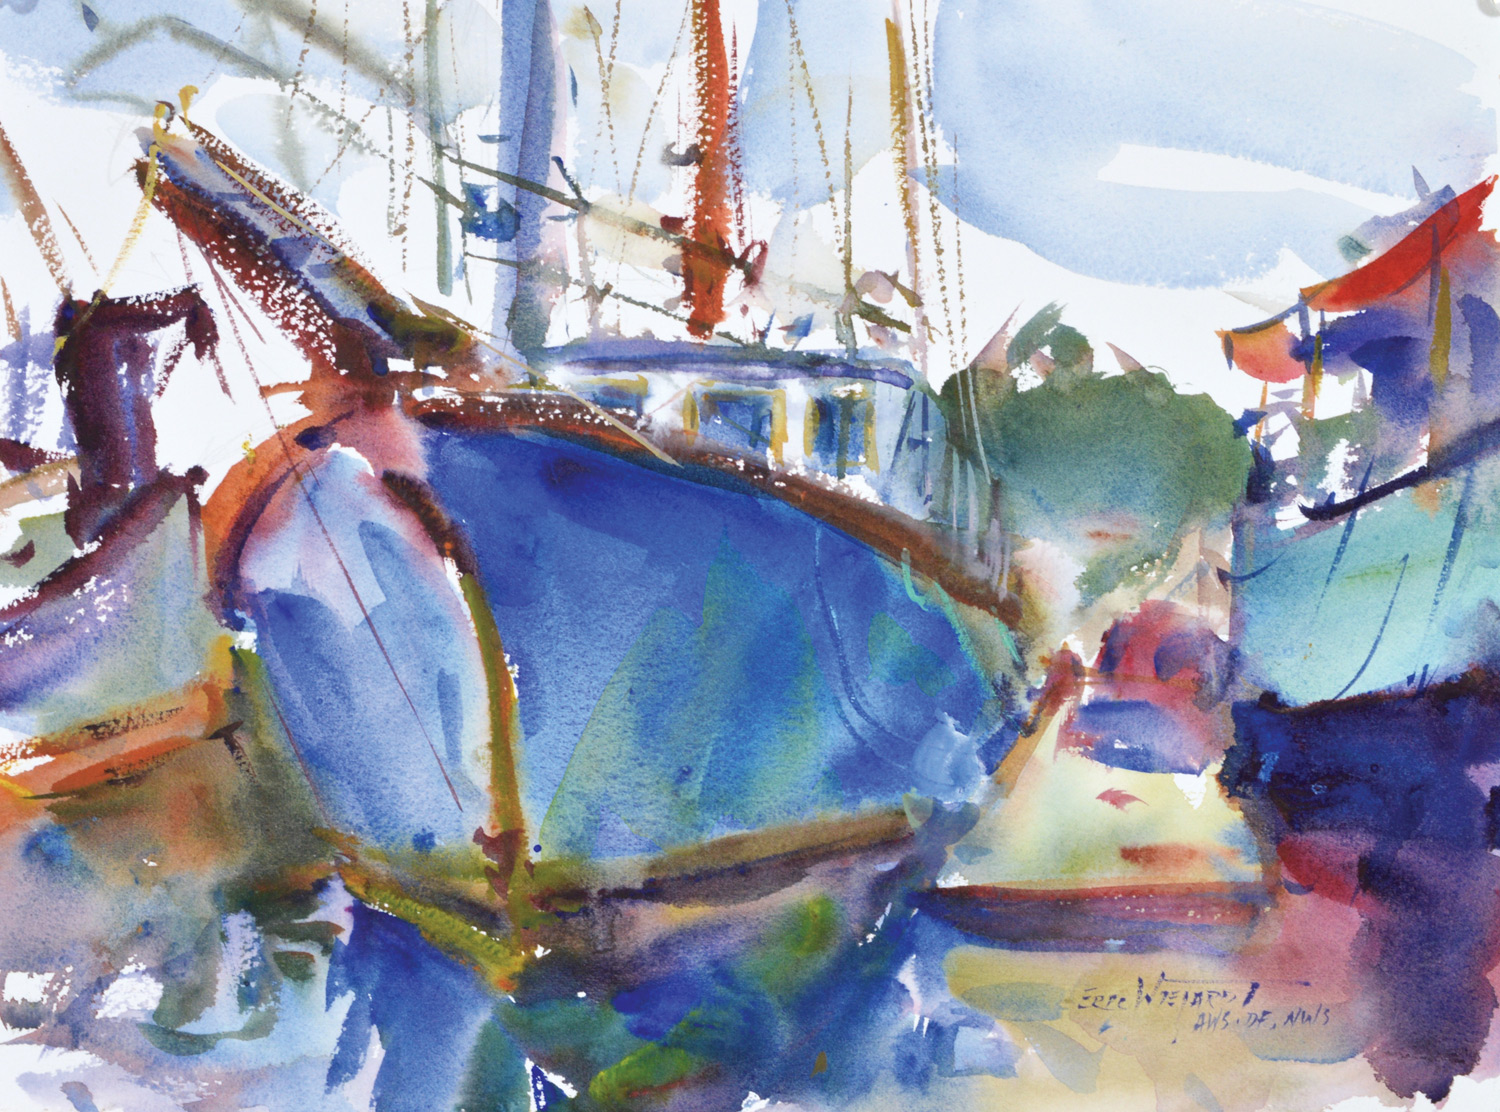
\includegraphics[scale=0.1]{image/watercolor.jpg}
        \caption{example Watercolor}
    \end{center}
\end{figure}

\subsection*{How will we do it}

The splats used will be created with procedural noise in order to not have the same splat. We have to play with the transparency to have this effect of water and wet effect. These splats will be placed by a noise with low frequency and less convolution has possible.

\section{Pointillism}

\subsection*{Description}

This technique consists to paint with only spots of different color.

\begin{figure}[!ht]
    \begin{center}
        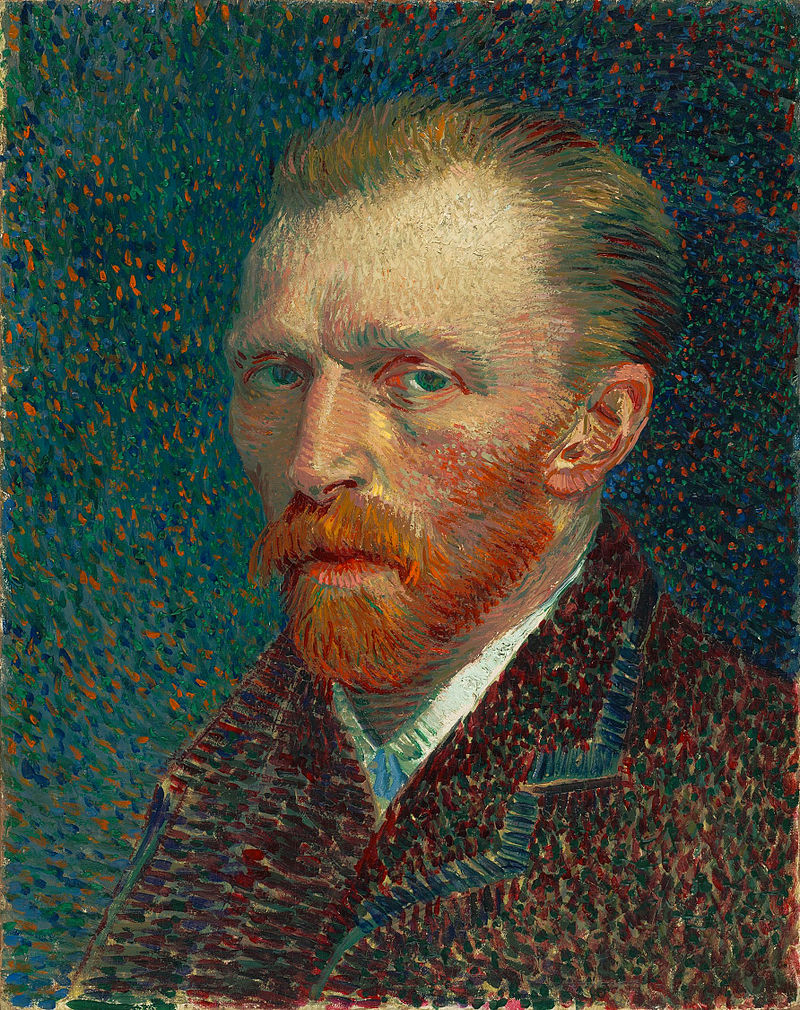
\includegraphics[scale=0.15]{image/VanGogh.jpg}
        \caption{example Pointillism}
    \end{center}
\end{figure}

\subsection{What makes a pointillism images?}

Is there space between dots ?


\subsection*{How will we do it}

The splats will be simple dot or many dots that will placed with a medium/high frequency.

\section{Hatching}

\subsection*{Description}

The technique consists to paint/draw with straight lines.

\begin{figure}[!ht]
    \begin{center}
        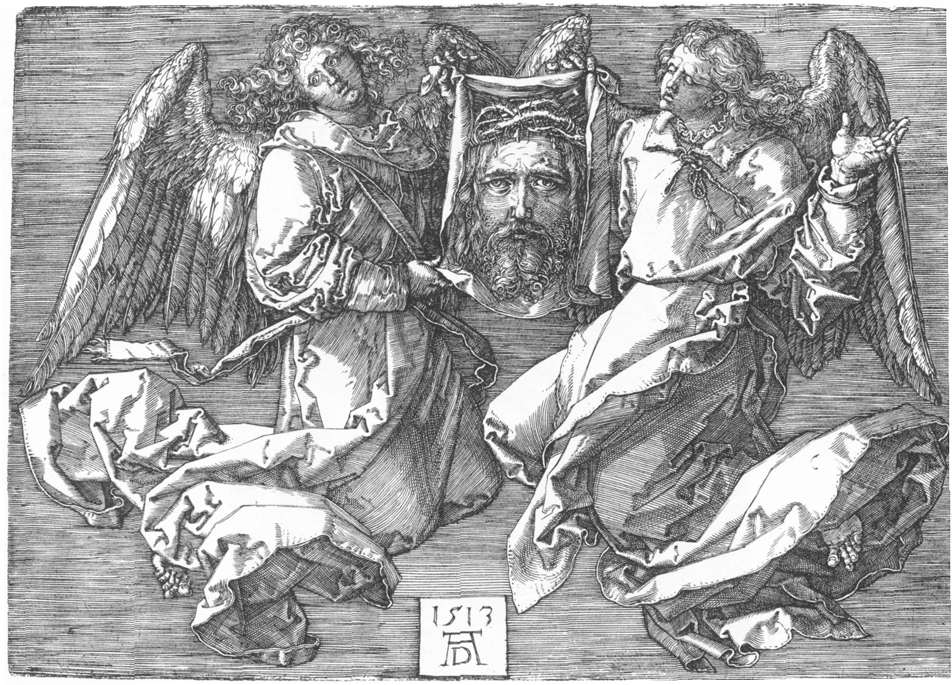
\includegraphics[scale=0.6]{image/hatching.jpg}
        \caption{example Hatching}
    \end{center}
\end{figure}

\subsection*{How will we do it}

The splats will be just one line or many lines. The noise will be at medium/high frequency.

\section{Classic painting}

\subsection*{Description}

This technique consists in drawing with a paintbrush.

\begin{figure}[!ht]
    \begin{center}
        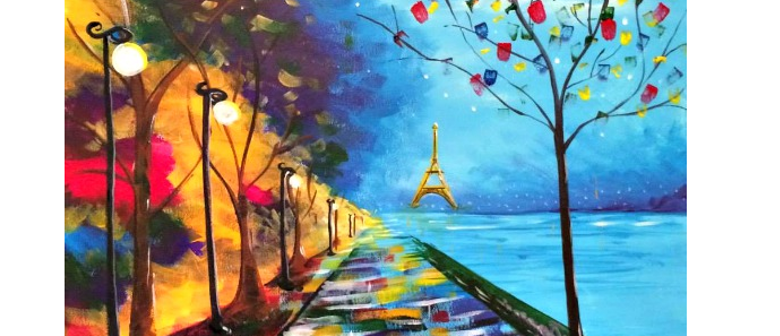
\includegraphics[scale=0.6]{image/paintbrush.png}
        \caption{example of painting with paintbrushes}
    \end{center}
\end{figure}

\subsection*{How will we do it}

The splats can be a brush stroke or it can be many. The noise to place these splats will i think be not too dense but it will depends on the size of the stroke in the splat.

\section{Hair drawing}

\subsection*{Description}

This technique has the goal to realise hairs in a painting/drawing.

\begin{figure}[!ht]
    \begin{center}
        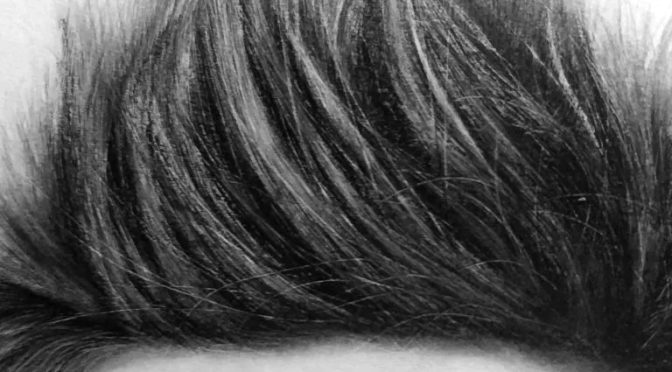
\includegraphics[scale=0.3]{image/hairs.jpg}
        \caption{example of hairs}
    \end{center}
\end{figure}

\subsection{How will we do it}

The splats can be one hair and the convolution will give the impression of hairs. Or the splats can be many hairs and so the noise needed will be at less frequency than the one with one hair per splat. We have to play with the size of the splats try to vary that and we have to adapted the orientation of the splat to have the impression that the splat is fix to the surface.

\section{Stippling}

\subsection*{Description}

The technique consists to paint with dots and to put an high density when the color is dark and few dots when the color is light.

\begin{figure}[!ht]
    \begin{center}
        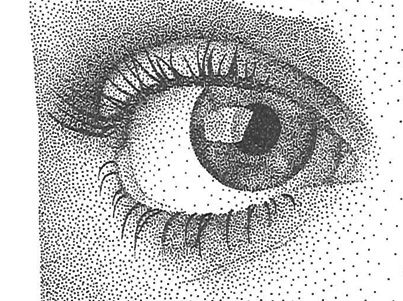
\includegraphics[scale=0.5]{image/stippling.jpg}
        \caption{example of stippling}
    \end{center}
\end{figure}

\subsection*{How will we do it}

The splat can be simple dot or many dots. We can also combine different splat and choosed with the darker of the color.

\end{document}
